\chapter{Fundamentação Teórica}

Neste capítulo serão apresentados os aspectos teóricos de lesões de pele, \acp{MLLM} e do \ac{LLaMA}-3.2. O funcionamento e desenvolvimento de \acp{MLLM} serão
esclarecidos com a explicação dos principais componentes desses modelos.

\section{Lesões de Pele}

A pele é o maior órgão do corpo humano e é responsável por proteger o corpo de agentes microbiológicos, físicos e químicos. Além disso, ela também ajuda na regulação da
temperatura do corpo e, através de receptores cutâneos, proporciona informações sensoriais como o tato \cite{skin}.

Devido à exposição da pele ao ambiente, é mais comum que esse órgão sofra com doenças. As áreas afetadas são consideradas lesões de pele e podem ser usadas para
diagnósticos de doenças \cite{segmentation_skin_lesions}.

Muitas doenças de pele se manifestam como lesões básicas que podem ser chamadas de lesões primárias. Vários fatores influenciam no diagnóstico de uma doença de pele,
\textcite{habif2015clinical} recomenda que sejam considerados aspectos como o histórico da lesão, distribuição, características visuais e testes laboratoriais. Porém,
o diagnóstico de uma doença de pele ainda é desafiador. Uma mesma doença de pele pode apresentar diferentes sintomas em cada instância e também pode evoluir ao longo do
tempo. A análise visual é o principal componente no diagnóstico de lesões de pele, nesse processo, a lesão é analisada pelas suas características superficiais, como a
cor, textura e presença de certas estruturas.

Uma doença que causa lesões de pele comumente estudada é o câncer de pele. Devido a sua relevância, será dada uma atenção maior a essa doença nesse trabalho.

\subsection{Câncer de Pele}

O câncer é uma doença caracterizada pela multiplicação de células anormais que podem se espalhar para além do seu tecido de origem, causando tumores e levando
eventualmente à morte \cite{cancer}. O câncer de pele é o tipo mais comum da doença globalmente e é mais frequentemente causado pela exposição prolongada à radiação
ultravioleta \cite{skin_cancer}. Em geral, essa doença afeta mais a pele clara e pode afetar a mesma pessoa mais de uma vez. Uma vez desenvolvido, há um aumento de 35\%
no risco de desenvolvimento de um novo câncer de pele do mesmo tipo em um período de três anos \cite{skin_cancer_zink}.

Existem várias categorias de câncer de pele, elas podem ser agrupadas como \ac{CPNM} e melanoma. \ac{CPNM} podem ser subdivididos em \ac{CBC}, \ac{CEC}, carcinoma de
Merkel e entre outros. Os \ac{CPNM} são os mais incidentes, correspondendo a mais de 90\% dos cânceres diagnosticados, e também são os menos fatais. O subtipo \ac{CBC} é o
mais frequente e corresponde a mais de 75\% dos casos de \ac{CPNM} no Brasil \cite{skin_cancer_zink}. O melanoma é o tipo mais fatal e menos incidente da doença. Cerca
de 75\% das mortes por câncer de pele são causadas por melanomas \cite{skin_cancer_screening}.

A doença tem um prognóstico muito melhor quando a detecção e tratamento são feitos cedo o suficiente. Segundo \textcite{skin_cancer_survival}, a taxa de sobrevivência ao
melanoma no Brasil é menor que a taxa global, sendo que há uma prevalência maior de casos avançados.

\subsection{Imagens de Lesões de Pele} \label{sec:skin_lesion_images}

As imagens para exames dermatológicos podem ser agrupadas em diferentes categorias. Alguns exemplos baseados em procedimentos recomendados por
\textcite{fotos_dermatologia} são:

\begin{itemize}
      \item \textbf{Dermatoscopia} (\autoref{fig:contact_pic}): Essas imagens são obtidas com um equipamento especializado, o dermatoscópio. Esse método permite que um
            diagnóstico mais preciso seja feito, sendo melhor que o olho nu na detecção de melanomas \cite{dermatoscopy};
      \item \textbf{Foto de aproximação com régua} (\autoref{fig:approximation_pic}): Esse tipo de imagem é obtida com uma fotografia feita a 30 centímetros da lesão,
            sem utilizar \textit{zoom}. Nessas imagens, etiquetas são colocadas próximas à lesão para auxiliar na determinação do seu tamanho;
      \item \textbf{Foto panorâmica} (\autoref{fig:panoramic_pic}): Nesse método são registradas imagens de regiões do corpo, como da cabeça, tronco, braços e pernas.
\end{itemize}

% TODO: Colocar a descrição longa e curta
\begin{figure}[ht]
      \centering
      \begin{minipage}{0.32\textwidth}
            \centering
            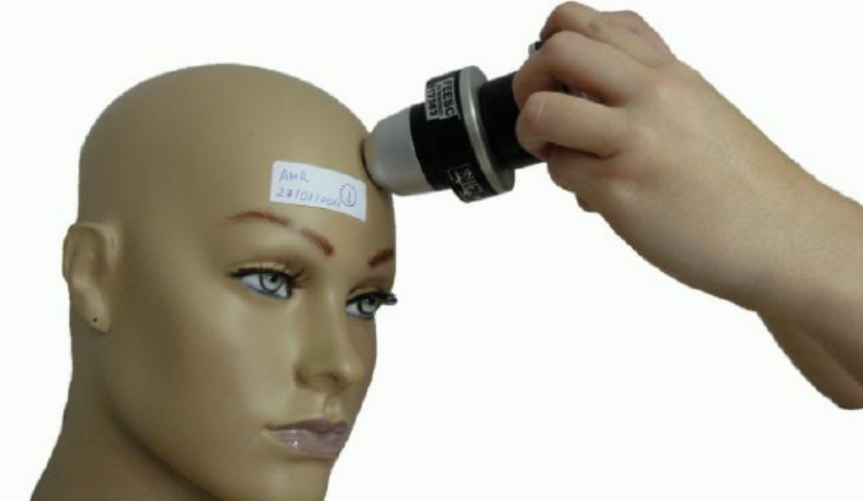
\includegraphics[height=0.8\columnwidth,keepaspectratio]{images/contact.png}
            \caption{\small Exemplo de exame com dermatoscopia. Fonte: \textcite{fotos_dermatologia}.}
            \label{fig:contact_pic}
      \end{minipage}\hfill
      \begin{minipage}{0.32\textwidth}
            \centering
            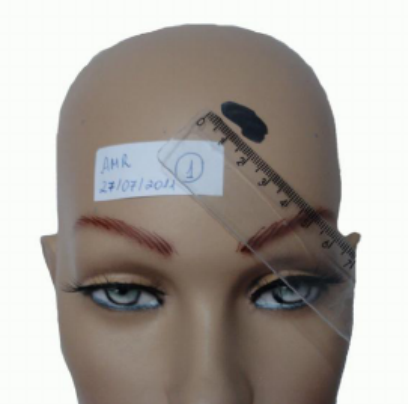
\includegraphics[height=0.8\columnwidth,keepaspectratio]{images/approximation.png}
            \caption{\small Exemplo de exame com aproximação. Fonte: \textcite{fotos_dermatologia}.}
            \label{fig:approximation_pic}
      \end{minipage}\hfill
      \begin{minipage}{0.32\textwidth}
            \centering
            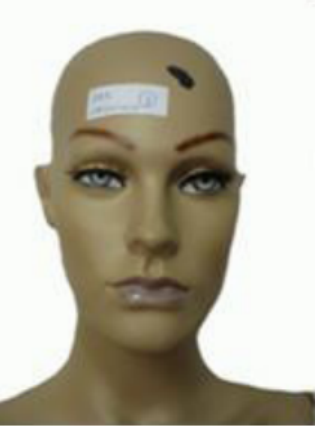
\includegraphics[height=0.8\columnwidth,keepaspectratio]{images/panoramic.png}
            \caption{\small Exemplo de exame com panorâmica da cabeça. Fonte: \textcite{fotos_dermatologia}.}
            \label{fig:panoramic_pic}
      \end{minipage}
\end{figure}

% TODO: Mudar para "Detecção e Diagnóstico de Lesões de Pele"
% TODO: Falar das técnicas atuais, por exemplo, ABCD
% TODO: Falar do processamento de imagens
% TODO: Falar da segmentação
% TODO: Falar da extração de características
% TODO: Falar da classificação de lesões
\subsection{Detecção e Diagnóstico de Câncer de Pele}

O câncer de pele pode ser identificado e classificado através dos sintomas causados. Características como o tamanho da lesão, variação da cor, irregularidade do formato,
progresso ao longo do tempo e local do corpo em que a lesão se encontra são fundamentais para o diagnóstico da doença \cite{recognizing_skin_cancer}.

A análise desses sintomas é normalmente um processo visual realizado por um dermatologista, sendo que técnicas como a dermatoscopia e teledermatologia podem ser usadas.
Outros métodos não invasivos incluem, por exemplo, a análise intracutânea espectrofotométrica, ultrasonografia de alta frequência e microscopia confocal de refletância.
É possível também diagnosticar a doença através de métodos invasivos como a biópsia. Além destes métodos, há também a utilização de \ac{IA}. Soluções com \ac{IA}
utilizam imagens para a classificação da doença e podem ter uma precisão equiparável ou até maior à de dermatologistas \cite{recognizing_skin_cancer, skin_cancer_ai}.

\section{Multimodal Large Language Models}

\acp{MLLM} são \acp{IA} baseadas em \acp{LLM} que possuem a capacidade de interpretação de diferentes modalidades de informação, diferentemente de \acp{LLM}, que
operam sobre informações textuais. Esses modelos também podem ser capazes de produzir conteúdo multimodal. Essas modalidades podem ser imagens, vídeos, áudios e
entre outros \cite{mllm_survey_2023, mllm_survey_2024}.

Segundo \textcite{mllm_survey_2024}, a estrutura de um \ac{MLLM} pode ser dividida em cinco componentes, sendo eles o codificador de modalidade, projetor de entrada,
\ac{LLM}, projetor de saída e o gerador de modalidade. No caso de \acp{MLLM} que possuem apenas saída de texto, só os três primeiros componentes estão presentes,
essa estrutura é demonstrada na \autoref{fig:mllm_structure_encoder_only}.

% TODO: Fazer uma figura melhor
\begin{figure}[ht]
      \centering
      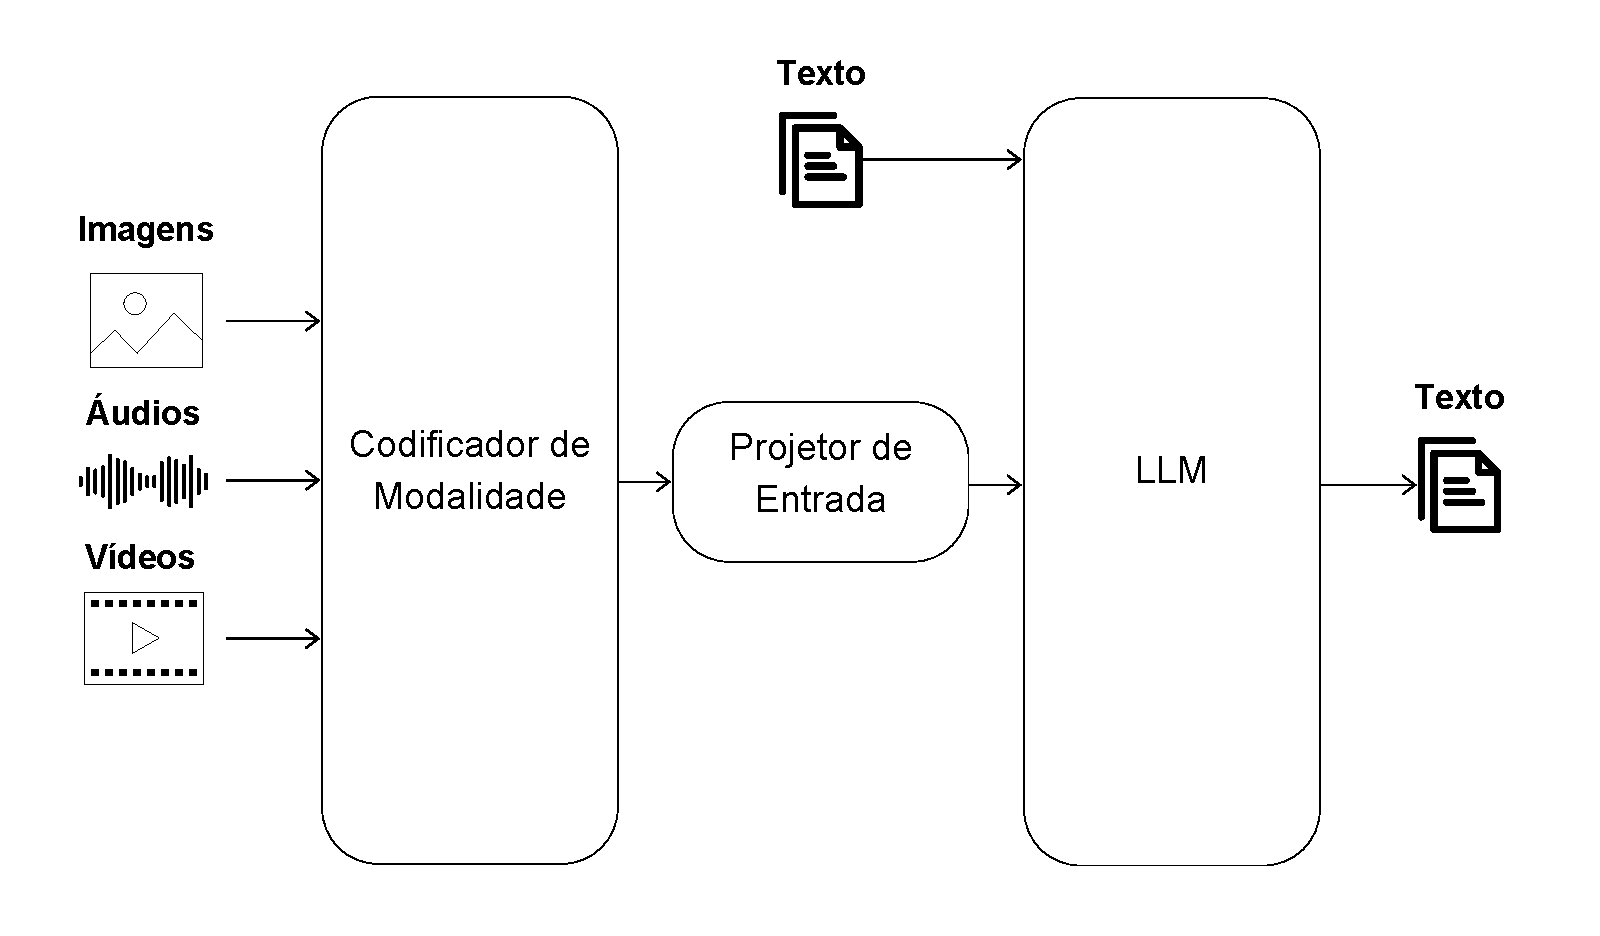
\includegraphics[width=0.7\columnwidth,keepaspectratio]{images/mllm_structure_encoder_only.pdf}
      \caption{\small Estrutura de um \ac{MLLM} que realiza apenas a interpretação multimodal.}
      \label{fig:mllm_structure_encoder_only}
\end{figure}

Neste trabalho, o foco será dado a modelos que interpretam imagens e retornam saídas textuais. Sendo assim, a parte de geração multimodal não será coberta.

\subsection{Large Language Models}

\acp{LLM} ou Grandes Modelos de Linguagem são modelos estatísticos pré-treinados baseados em transformadores que possuem bilhões de parâmetros e conseguem processar e
gerar textos em linguagem natural \cite{llm_survey_2024}.

Embora modelos de linguagem já sejam conceitos discutidos há várias décadas, a introdução da arquitetura de transformadores no artigo \textit{Attention Is All You Need}
de \textcite{transformer} define um marco no desenvolvimento destes modelos, levando ao surgimento de \acp{LLM}.

Transformadores foram desenvolvidos inicialmente para tarefas de tradução. Porém, pouco tempo depois da sua introdução, pesquisadores da OpenAI aplicaram essa arquitetura
no desenvolvimento do modelo \ac{GPT}, que demonstrou características emergentes além da simples geração de texto, como a capacidade de responder perguntas com
respostas que não estavam na sua base de treinamento \cite{gpt1}. Os modelos sucessores, \ac{GPT}-2 e \ac{GPT}-3, demonstraram ser ainda melhores em diversas tarefas,
como a tradução, resolução de problemas básicos, interpretação de texto e aritmética básica \cite{gpt2, gpt3}.

Após o lançamento comercial do \textit{ChatGPT} em 2022, vários novos \acp{LLM} foram desenvolvidos. Os mais notáveis são baseados no \ac{LLaMA} e no \ac{PaLM}
\cite{llm_survey_2024}.

As próximas subseções tratarão dos conceitos da representação do texto de entrada, como a tokenização, o uso de \textit{embedding vectors} ou incorporações vetoriais e
codificação posicional. Depois, a arquitetura de transformadores será explicada.

\subsubsection{Tokenização}

A tokenização é um processo em que o texto é separado em partes menores, denominados \textit{tokens}. A maioria das formas de tokenização quebram palavras em
sub-palavras, isso permite que o modelo interprete novas palavras não vistas antes com base na composição das sub-palavras. Esse processo também torna o processamento de
texto mais eficiente, reduzindo a memória necessária para o vocabulário \cite{tokenizer_performance}. Na \autoref{fig:tokens} é possível ver um exemplo de texto
tokenizado. Cada preenchimento colorido denota um \textit{token}.

\clearpage

\begin{figure}[ht]
      \centering
      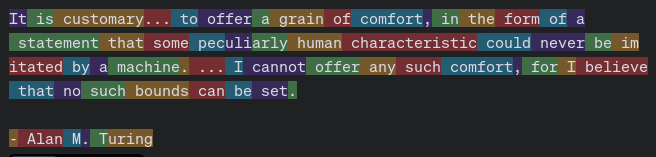
\includegraphics[width=0.7\columnwidth,keepaspectratio]{images/tokens.png}
      \caption{\small Texto tokenizado com o tokenizador do \ac{GPT}-4o. Fonte: \textcite{tokenizer}.}
      \label{fig:tokens}
\end{figure}

O mesmo texto, representado como uma lista de \textit{IDs} de \textit{tokens} pode ser visto na \autoref{fig:tokens_ids}.

\begin{figure}[ht]
      \centering
      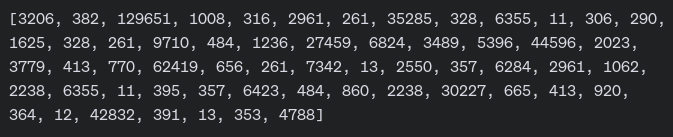
\includegraphics[width=0.7\columnwidth,keepaspectratio]{images/tokens_ids.png}
      \caption{\small \textit{IDs} de \textit{tokens} gerados com o tokenizador do \ac{GPT}-4o. Fonte: \textcite{tokenizer}.}
      \label{fig:tokens_ids}
\end{figure}

\textcite{llm_survey_2024} elenca os tipos mais comuns de tokenização, sendo eles o \textit{Byte pair encoding}, \textit{Word piece encoding} e
\textit{Sentence Piece Encoding}:

\begin{itemize}
      \item \textbf{\textit{Byte pair encoding}}: Neste algoritmo o texto é quebrado com base na frequência das palavras. Palavras mais frequentes se mantém inteiras
            enquanto as menos frequentes são quebradas;
      \item \textbf{\textit{Word piece encoding}}: No \textit{Word piece encoding}, o algoritmo é inicializado com o alfabeto da linguagem e depois passa por uma etapa
            de treinamento, onde os caracteres são combinados em sub-palavras com base na frequência em que elas aparecem. O treinamento continua até que toda a base
            textual possa ser representada com o vocabulário de \textit{tokens};
      \item \textbf{\textit{Sentence Piece Encoding}}: Este método é similar aos já citados, porém, sua maior diferença está na forma em que o texto é tratado. Sendo
            que o texto é dado como uma sequência contínua de caracteres, sem assumir que delimitações existam entre as palavras. Isso se torna útil na tokenização de
            línguas sem delimitações com espaços, como, por exemplo, japonês e chinês.
\end{itemize}

\subsubsection{Incorporação Vetorial}

Uma incorporação vetorial é um vetor de valores reais em um espaço semântico n-dimensional que representa um dado, como, por exemplo, uma palavra ou uma imagem. Esse
tipo de representação permite que diferentes tipos de dados sejam representados em um espaço vetorial unificado. Na \autoref{fig:word_embeddings} há um exemplo
simplificado da estrutura destes vetores. No contexto de \acp{LLM}, \textit{tokens} são representados com incorporações vetoriais \cite{word_embedding, mllm_survey_2023}.

\begin{figure}[ht]
      \centering
      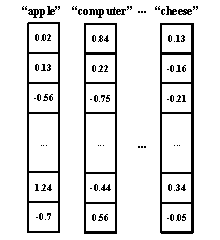
\includegraphics[width=0.3\columnwidth,keepaspectratio]{images/word_embeddings.pdf}
      \caption{Representação de palavras como vetores de valores reais. Fonte: \textcite{word_embedding}.}
      \label{fig:word_embeddings}
\end{figure}

Nesse espaço vetorial, direções podem ter um significado semântico. Um exemplo dado por \textcite{glove} demonstra isso com a frase \textit{``king is to queen as man is
      to woman''}, que pode ser representada como \begin{math}V_{king} - V_{queen} \approx V_{man} - V_{woman}\end{math}, evidenciando que a direção do vetor
\begin{math}V_{king} - V_{queen}\end{math} codifica informações sobre gênero. A \autoref{fig:word_embeddings_directions} traz uma visualização aproximada desta relação.

\begin{figure}[ht]
      \centering
      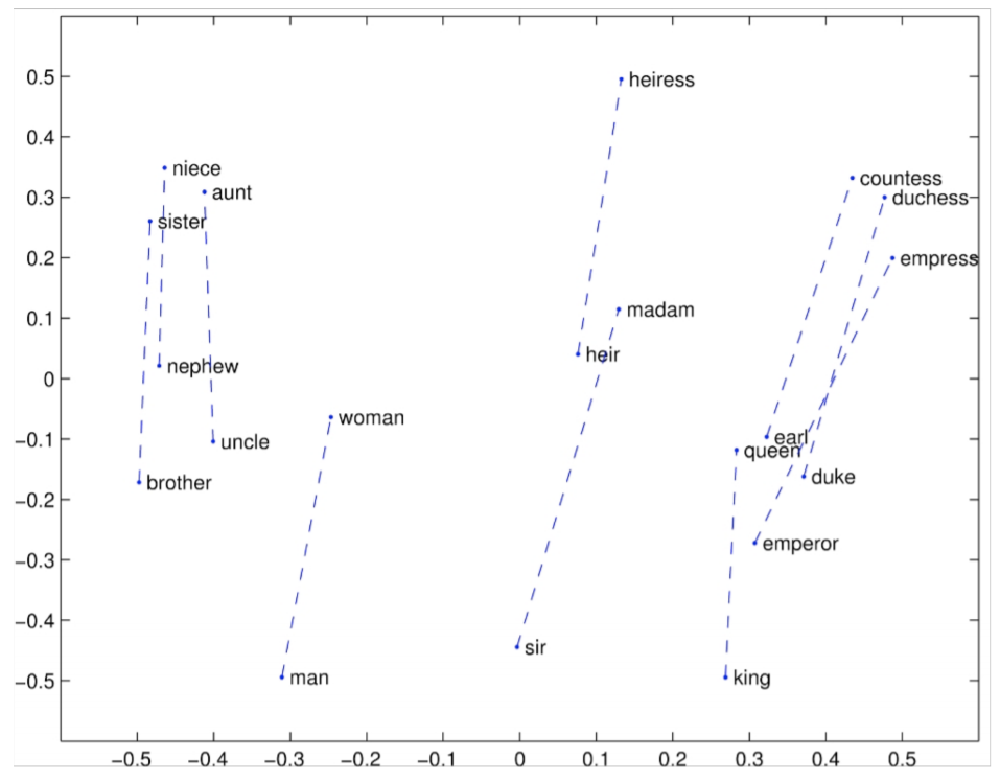
\includegraphics[width=0.6\columnwidth,keepaspectratio]{images/word_embeddings_directions.png}
      \caption{Visualização aproximada de incorporações com a direção que codifica informações de gênero evidenciada. Fonte: \textcite{word_embedding}.}
      \label{fig:word_embeddings_directions}
\end{figure}

Outro exemplo de relação semântica pode ser visto com \begin{math}V_{Paris} - V_{France} + V_{Italy} \approx V_{Rome}\end{math}, em que é possível calcular qual é a
capital da Itália somando um vetor que incorpora a relação de capital para país com um vetor que incorpora a palavra ``Itália''. A proximidade entre incorporações indica
a similaridade semântica entre elas \cite{word2vec_estimation}.

\subsubsection{Codificação Posicional}

Transformadores não possuem mecanismos de recorrência ou convolução, então é necessária uma forma de codificar a posição de cada \textit{token} do texto de entrada. No
modelo original de transformador, isso foi feito com a adição de vetores de codificação posicional às incorporações. Para gerar uma codificação como esta, é usada uma
combinação de funções seno e cosseno com diferentes frequências, sendo que cada dimensão da codificação corresponde a um senoide \cite{transformer}. A
\autoref{fig:absolute_positional_embeddings} apresenta uma visualização das codificações posicionais com o método utilizado no transformador original.

\begin{figure}[ht]
      \centering
      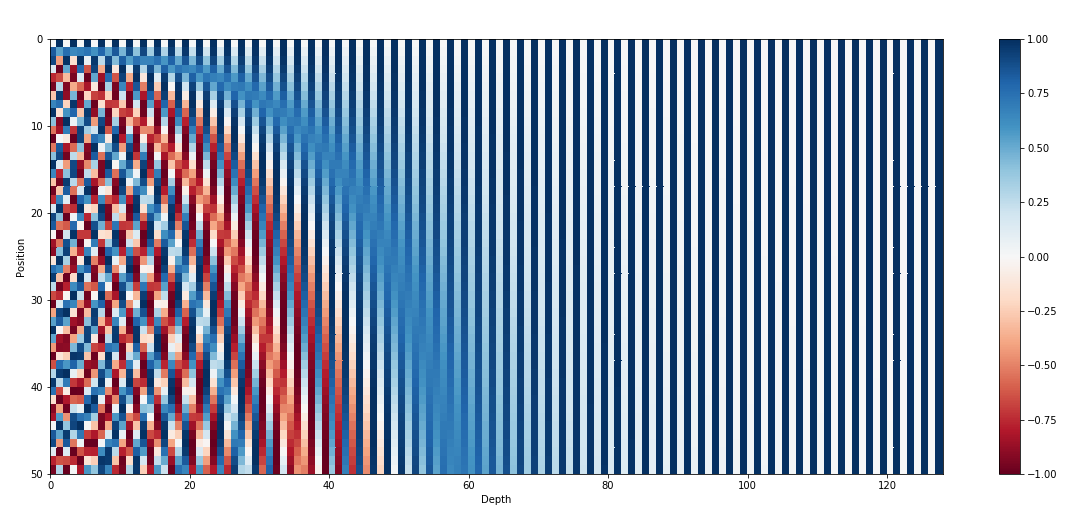
\includegraphics[width=1.0\columnwidth,keepaspectratio]{images/absolute_positional_embeddings.png}
      \caption{Visualização da codificação posicional original, cada faixa horizontal corresponde a uma incorporação. Fonte: \textcite{positional_embeddings}.}
      \label{fig:absolute_positional_embeddings}
\end{figure}

% TODO: Verificar porquê o RoPE não aparece na versão longa sem forçar
Essa forma de codificação é conhecida como \ac{APE}, ela possui certas desvantagens, como a limitação no número de incorporações e a incapacidade de reconhecer
distâncias relativas. Mas, existem outras formas de codificação que lidam com esses problemas, como \ac{RPE}, \acl{RoPE} e vieses posicionais relativos.
\textcite{llm_survey_2024} traz definições sobre esses outros tipos:

\begin{itemize}
      \item \textbf{\ac{RPE}}: Nessa forma de codificação, os \textit{tokens} são representados em pares ligados entre si, tornando a entrada do modelo em um grafo
            dirigido conexo. Esse método é implementado diretamente no mecanismo de atenção do transformador. Porém, o \ac{RPE} tem a desvantagem de tornar o treinamento
            e a inferência mais lentos, devido à modificação do mecanismo de atenção;
      \item \textbf{\ac{RoPE}}: Essa codificação aplica uma rotação no ângulo \begin{math}m\theta\end{math} nos pares de vetores de
            \textit{query} e \textit{key}\footnote{Esses vetores serão explicados na \autoref{sec:transformers}}, sendo que \begin{math}\theta\end{math} é um ângulo
            pré-definido e \begin{math}m\end{math} é o índice da posição absoluta do vetor de incorporação usado para gerar os vetores de \textit{query} e \textit{key}. O
            esquema do \ac{RoPE} pode ser visto na \autoref{fig:rotary_positional_embeddings};
      \item \textbf{Vieses posicionais relativos}: Nesse método, são introduzidos vieses no nível de atenção calculada entre cada \textit{query} e \textit{key},
            penalizando os pares que estiverem distantes entre si.
\end{itemize}

\begin{figure}[ht]
      \centering
      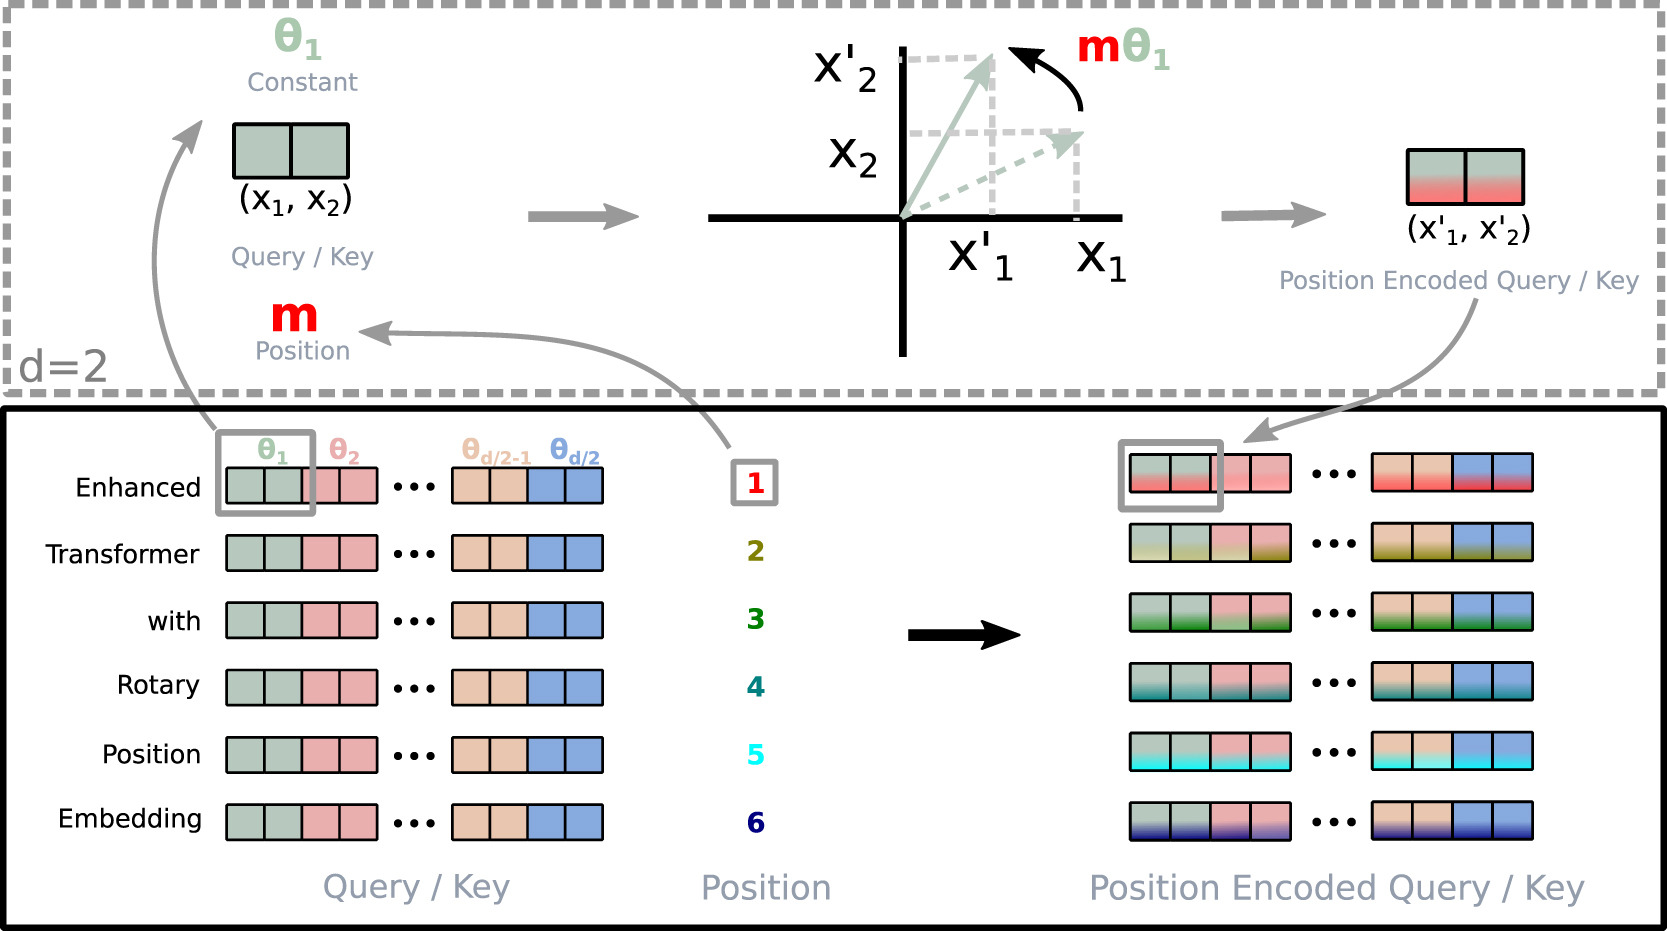
\includegraphics[width=0.8\columnwidth,keepaspectratio]{images/rotary_positional_embeddings.jpg}
      \caption{Funcionamento da codificação do tipo \ac{RoPE}. Fonte: \textcite{su2024roformer}.}
      \label{fig:rotary_positional_embeddings}
\end{figure}

\subsubsection{Transformadores} \label{sec:transformers}

O transformador é o componente central de um \ac{LLM}, ele processa o texto de entrada previamente tokenizado e representado em incorporações vetoriais e prevê o
próximo \textit{token} desse texto. As explicações fornecidas neste trabalho se baseiam no modelo de \textcite{transformer}, mas várias outras variantes já existem.

A arquitetura original dos transformadores possui um codificador e um decodificador, sendo que cada um deles é composto por camadas. No codificador, cada camada é
composta por duas subcamadas, sendo uma delas um mecanismo de \textit{multi-head self-attention} e outra, uma rede \textit{feed-forward}. A saída de cada uma delas possui
uma conexão residual e uma etapa de normalização. O decodificador é similar ao codificador, mas suas camadas possuem uma subcamada extra que aplica o mecanismo de
\textit{multi-head self-attention} mascarado sobre a saída do codificador. Além disso, a entrada do decodificador é deslocada em uma posição, de modo que uma nova
incorporação possa ser prevista e usada para gerar um \textit{token}. A \autoref{fig:transformer} mostra o transformador original.

\begin{figure}[ht]
      \centering
      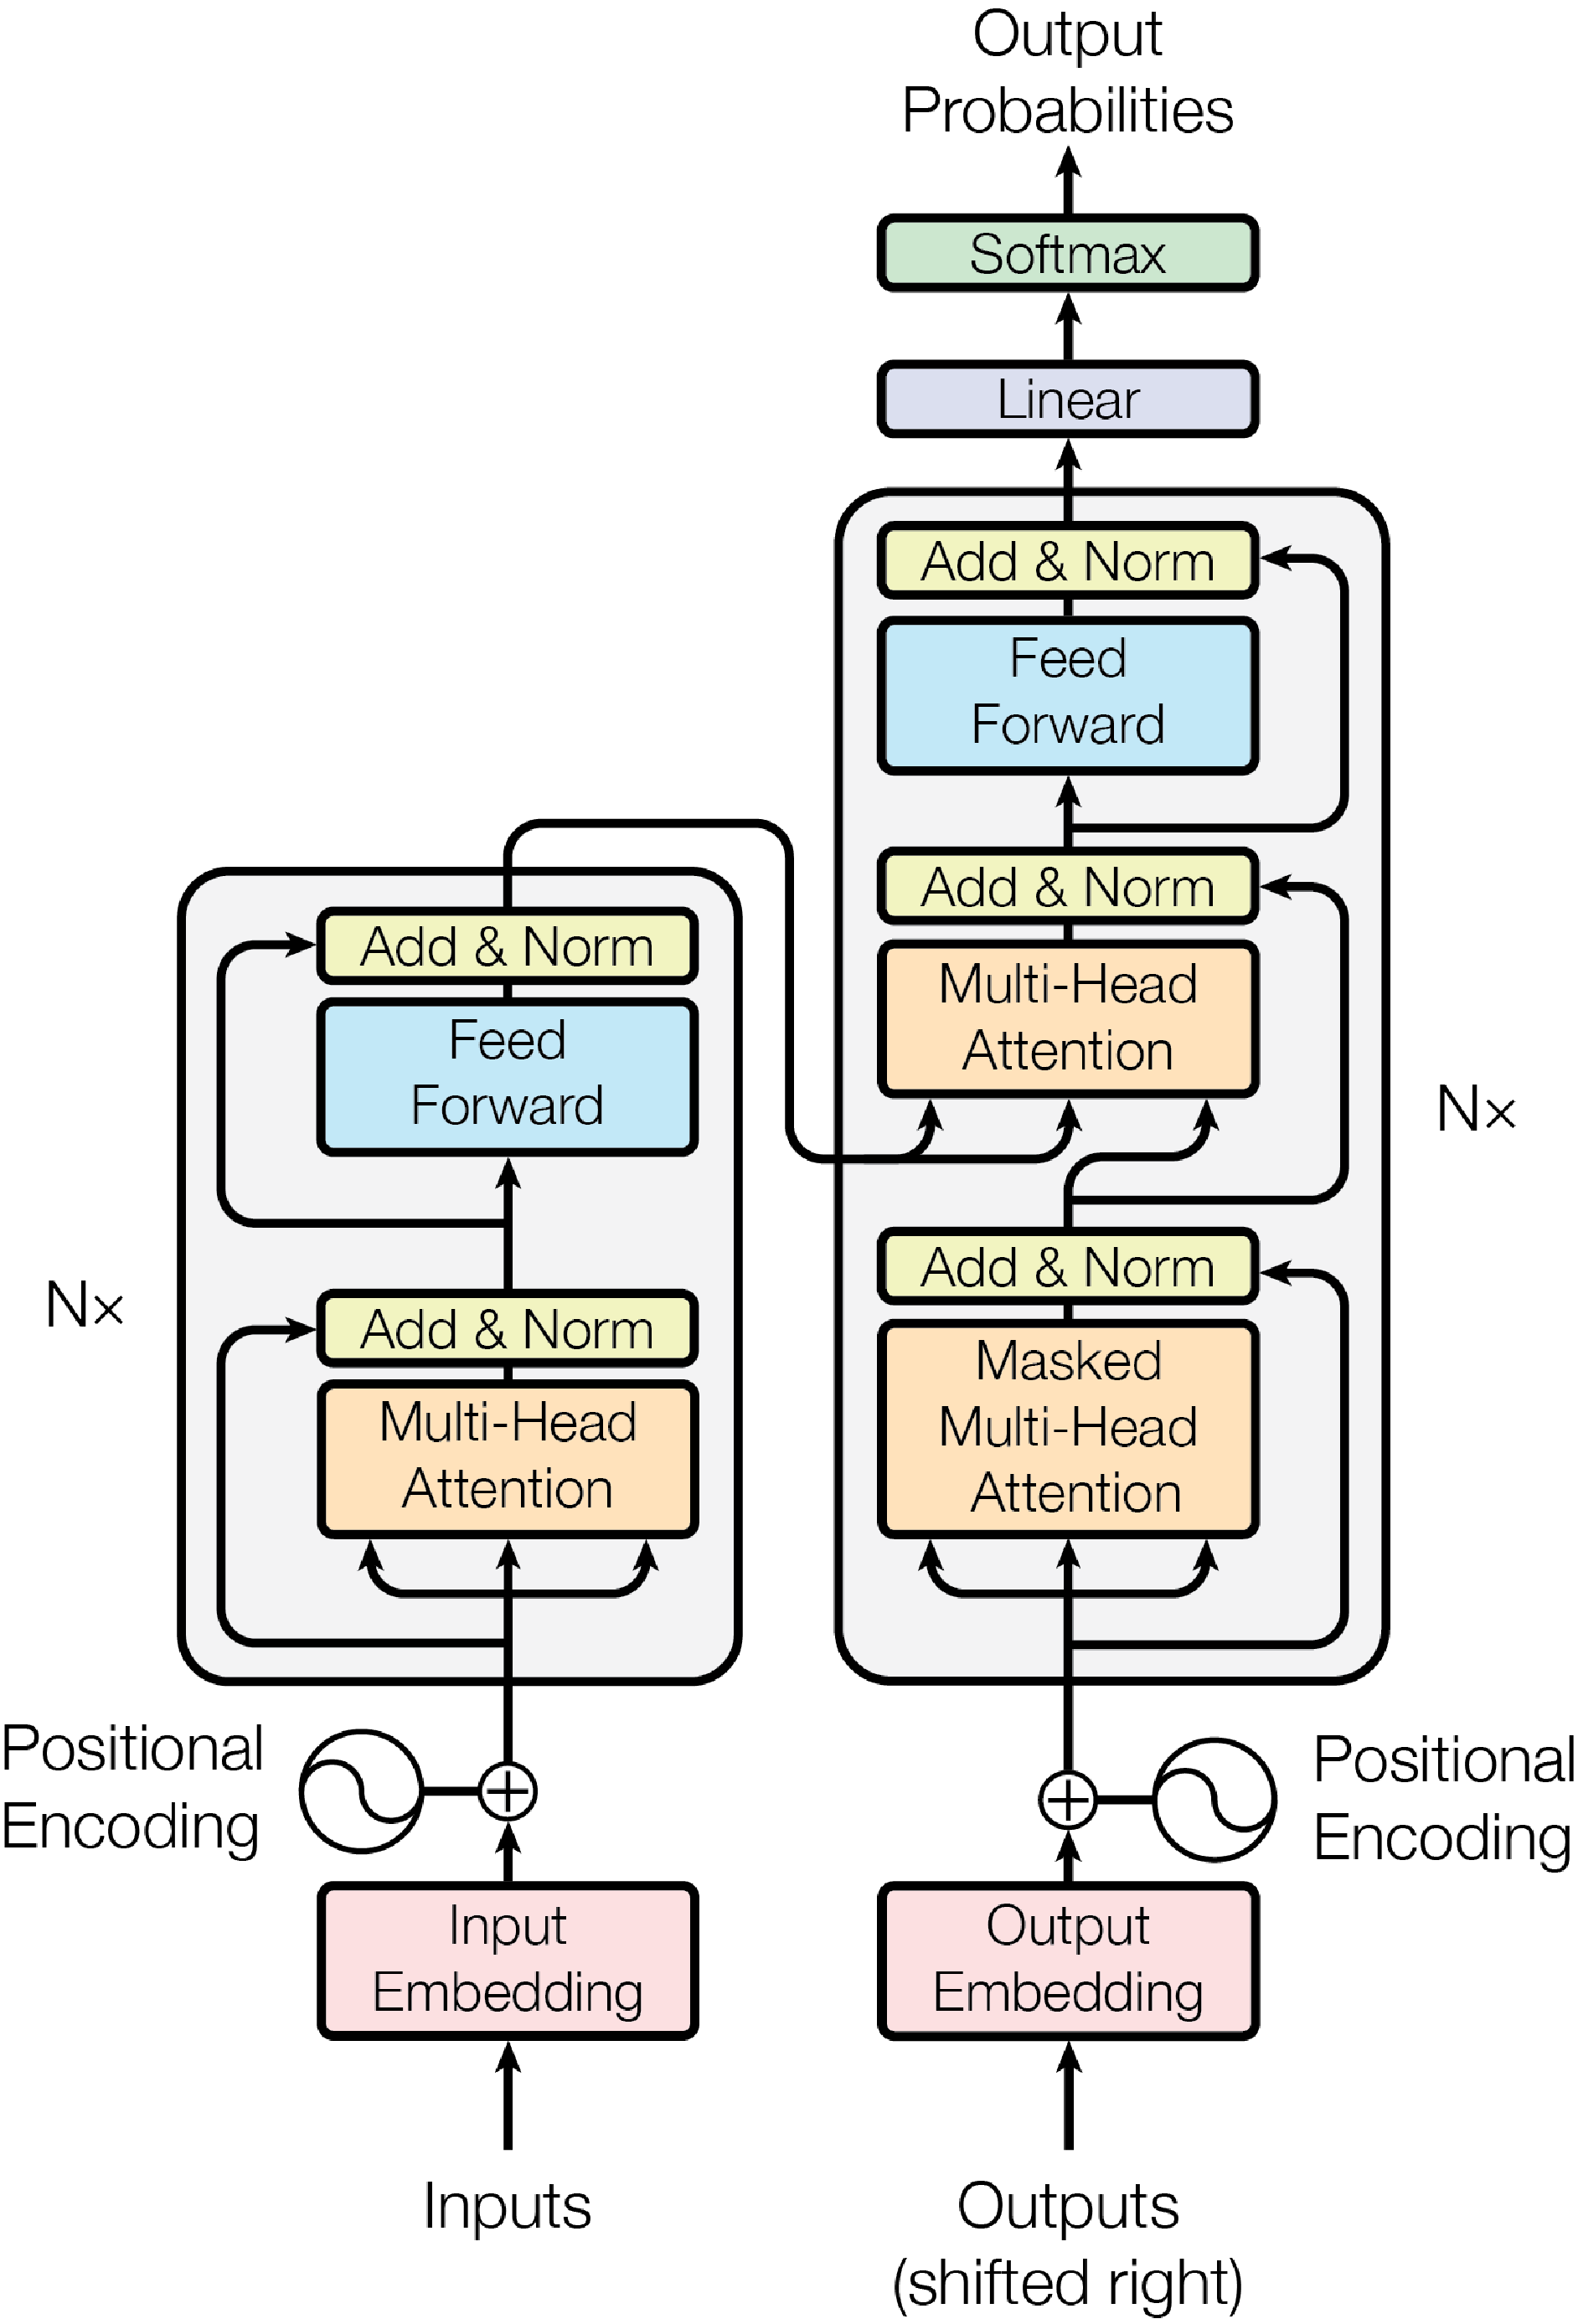
\includegraphics[width=0.4\columnwidth,keepaspectratio]{images/transformer.png}
      \caption{Arquitetura de um transformador. Fonte: \textcite{transformer}.}
      \label{fig:transformer}
\end{figure}

O mecanismo de \textit{multi-head self-attention} permite que o modelo reconheça as relações entre diferentes partes do texto de entrada e ajuste os valores das
incorporações vetoriais com base nessas relações. Esse conceito pode ser exemplificado de forma mais intuitiva com a frase: \textit{``Você está lendo um documento, ele
      foi escrito em português''}. Nesse caso, a palavra \textit{``ele''} possui uma relação com a palavra \textit{``documento''}. O mecanismo identificaria essa relação e
utilizaria essa informação para recalcular a incorporação vetorial da palavra \textit{``ele''}, de modo que ela reflita seu vínculo com \textit{``documento''}. A captura
das relações e significados é o que permite que o modelo gere mais partes do texto. Por exemplo, na frase \textit{``Um animal vivendo em seu habitat...''}, o modelo
poderia ajustar o valor semântico de uma nova incorporação com base na sua relação com outras incorporações até que ela representasse a palavra \textit{``natural''}.

O modelo de atenção proposto originalmente se chama \textit{Scaled Dot-Product Attention}. Na primeira etapa do processamento, são calculados três vetores para cada
incorporação vetorial, sendo eles o \textit{query} (\begin{math}V_Q\end{math}), \textit{key} (\begin{math}V_K\end{math}) e \textit{value} (\begin{math}V_V\end{math}).
Para realizar esta operação, as incorporações são agrupadas em uma matriz \begin{math}E\end{math} e multiplicadas pelas matrizes \begin{math}W_Q\end{math},
\begin{math}W_K\end{math} e \begin{math}W_V\end{math}, provenientes do treinamento do modelo. Assim, são obtidas as matrizes \begin{math}Q\end{math},
\begin{math}K\end{math} e \begin{math}V\end{math}. As equações abaixo ilustram este processo:

\begin{align*}
      E \times W_Q & = Q \\
      E \times W_K & = K \\
      E \times W_V & = V
\end{align*}

Além disso, os vetores nas matrizes \begin{math}Q\end{math} e \begin{math}K\end{math} possuem uma dimensionalidade menor do que os vetores de incorporação. Isso se dá
por uma escolha de desenvolvimento na arquitetura original que visava melhorar o desempenho no processamento da atenção \textit{multi-head}.

A próxima etapa se consiste no cálculo do produto escalar entre todos os vetores \begin{math}V_Q\end{math} com todos os \begin{math}V_K\end{math}, através da operação
\begin{math}Q \times K^T\end{math}. O valor resultante de cada produto indica o quanto um vetor \begin{math}V_K\end{math} atende a um \begin{math}V_Q\end{math}. Em
outras palavras, um produto escalar alto indica que o \textit{token} de onde foi calculado o \begin{math}V_K\end{math} tem uma relação com o \textit{token} de
onde foi calculado o \begin{math}V_Q\end{math}.

Os valores resultantes são divididos por \begin{math}\sqrt{d_k}\end{math}, garantindo uma maior estabilidade no gradiente de valores. Nesse caso,
\begin{math}d_k\end{math} é número de dimensões no espaço de \textit{queries} e \textit{keys}. Depois, uma função de \textit{softmax} é aplicada, normalizando os
resultados.

Por fim, os vetores da matriz \begin{math}V\end{math} são multiplicados pelos valores normalizados. Assim, vetores \begin{math}V_V\end{math} de \textit{tokens} com pouca
relação entre si serão numericamente irrelevantes. Depois, os vetores resultantes relativos a cada \textit{token} são somados, gerando novos vetores que representam o
ajuste no significado das incorporações vetoriais desses \textit{tokens}. O resultado desta etapa é uma matriz composta por esses vetores de ajuste.

O processo definido até o momento pode ser resumido com a expressão:

\begin{align*}
      Attention(Q, K, V) & = softmax({\frac{QK^T}{\sqrt{d_k}}})V
\end{align*}

O conceito de \textit{multi-head} é utilizado para melhorar a capacidade do modelo de dar atenção a diferentes partes do texto de entrada. Para cada cabeça há um
conjunto distinto de matrizes \begin{math}Q\end{math}, \begin{math}K\end{math} e \begin{math}V\end{math}. No fim, cada cabeça irá produzir um vetor de ajuste diferente
para cada \textit{token}. As matrizes de vetores de ajuste de cada cabeça são concatenadas e multiplicadas por uma matriz \begin{math}W_O\end{math}, gerando a saída da
subcamada de atenção. A expressão abaixo e a \autoref{fig:attention} demonstram o processo e a estrutura:

\begin{align*}
      MultiHead(Q, K, V) & = Concat(head_1,...,head_h)W_O
\end{align*}

\begin{figure}[ht]
      \centering
      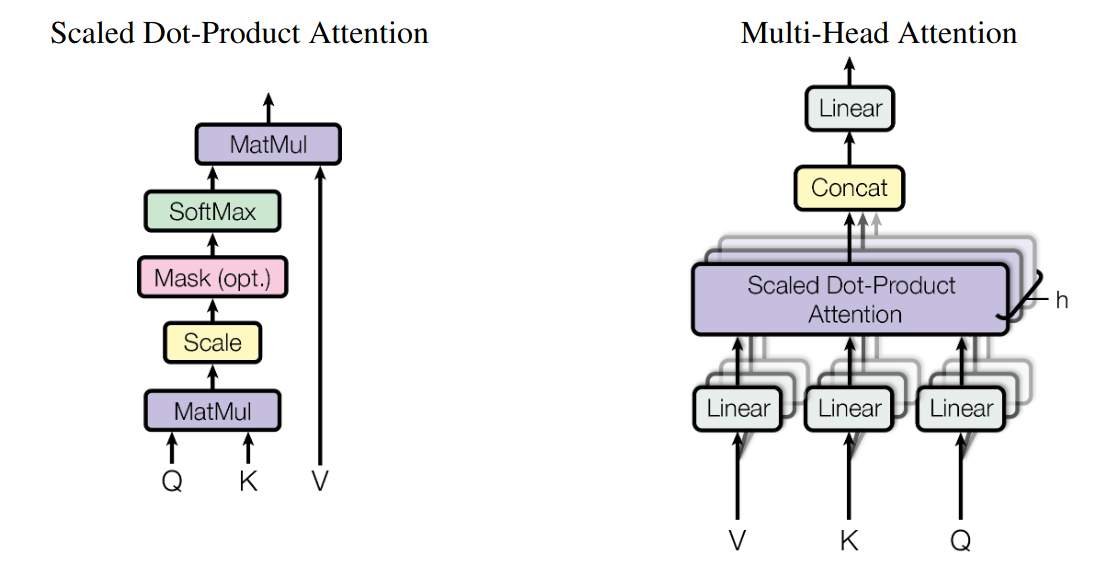
\includegraphics[width=0.7\columnwidth,keepaspectratio]{images/attention.png}
      \caption{Estrutura da subcamada de atenção. Fonte: \textcite{transformer}.}
      \label{fig:attention}
\end{figure}

A saída de cada subcamada possui uma conexão residual que soma os dados de entrada com os de saída dessa subcamada, aplicando uma normalização em seguida. Esse processo
atualiza as incorporações com os vetores de ajuste e também atenua o problema do desaparecimento de gradiente.

A próxima subcamada, a de \textit{feed-forward}, é composta por duas transformações lineares com uma função de ativação \ac{ReLU} entre elas. Cada incorporação é
processada isoladamente por esta subcamada. \textcite{feed_forward_knowledge} propõe que essa rede armazena as informações factuais aprendidas no treinamento. A
expressão abaixo traz a representação matemática desta subcamada:

\begin{align*}
      FFN(x) & = ReLU(xW_1+b_1)W_2 + b_2
\end{align*}

A saída do conjunto de camadas de codificação é utilizada pelas camadas de decodificação. No decodificador há uma subcamada extra de \textit{multi-head self-attention}
mascarada que processa os dados de uma forma em que cada incorporação só possa ser atendida pelas incorporações antecessoras a ela. Em outras palavras, o valor semântico
de um \textit{token} só pode ser influenciado pelos valores dos \textit{tokens} antecessores a ele. Isso é implementado com a definição do valor
\begin{math}-\infty\end{math} para as relações ilegais após a etapa de multiplicação e escala das matrizes \begin{math}Q\end{math} e \begin{math}K\end{math}, que é
normalizado como zero com a aplicação de \textit{softmax}. Com a aplicação desta máscara e do deslocamento da entrada do codificador em uma posição, é possível prever
uma nova incorporação vetorial que dependa apenas das incorporações anteriores.

Por fim, a nova incorporação prevista pelo decodificador passa por uma transformação linear que gera um vetor de \textit{logit}. O tamanho deste vetor está associado ao
tamanho do vocabulário de \textit{tokens} do modelo, sendo que cada posição sua corresponde a um \textit{token}. O \textit{logit} é normalizado com \textit{softmax},
gerando uma distribuição de probabilidades. O \textit{token} que corresponde ao valor com a maior probabilidade é então usado para completar o texto de entrada.

\subsubsubsection{Arquiteturas de Transformadores}

O modelo explicado anteriormente possui um codificador e decodificador, sendo mais complexo e adequado para tarefas de geração de texto com base em uma entrada específica,
como a geração de resumos ou a tradução. Existem também modelos que possuem apenas codificadores ou decodificadores. Os que usam apenas codificadores são úteis para
tarefas de classificação de texto, \ac{REM} e \ac{EQA}. Modelos que usam apenas decodificadores são mais utilizados para a geração de texto, sendo que os modelos das
famílias \ac{GPT} e \ac{LLaMA} são exemplos dessa forma de implementação \cite{llm_survey_2024}.

\subsection{Codificador de Modalidade}

Codificadores de modalidade são os componentes responsáveis pela extração das características mais relevantes dos dados multimodais de entrada em incorporações vetoriais.
\cite{mllm_survey_2024}. Este trabalho apresentará apenas a categoria visual de codificador.

\subsubsection{Codificador Visual}

Existem diversos codificadores visuais. Os mais comuns usam \acp{ViT} ou Transformadores Visuais nas suas arquiteturas, mas também há codificadores baseados em
convolução, como o \textit{Osprey} \cite{mllm_survey_2023}. Neste trabalho o foco será direcionado a arquiteturas baseadas em \ac{ViT}.

\subsubsubsection{Transformadores Visuais}

\acp{ViT} são transformadores capazes de processar imagens que foram introduzidos por \textcite{dosovitskiy2020image}. A arquitetura original utiliza apenas codificadores
e visa classificar imagens.

A primeira etapa no processamento envolve a divisão da imagem em seções de menor resolução, sendo então planificadas e incorporadas. Cada incorporação resultante também
recebe uma codificação posicional simples unidimensional. Nessa etapa, uma incorporação extra também pode ser adicionada na primeira posição da entrada para objetivos de
classificação de imagens.

Na próxima etapa, as incorporações são processadas pelo transformador, capturando suas relações e refinando-as. Diferentemente da arquitetura de \textcite{transformer},
o modelo de \textcite{dosovitskiy2020image} aplica a normalização antes da subcamada de atenção. Além disso, a função de ativação usada na subcamada de
\textit{feed-forward} é a \ac{GELU}.

A classificação pode ser realizada com o processamento da incorporação de classificação por um \ac{MLP}. Assim, é gerada uma distribuição de probabilidades sobre as
classes. A \autoref{fig:vision_transformer} demonstra a estrutura de um transformador visual com os detalhes de sua implementação.

\clearpage

\begin{figure}[ht]
      \centering
      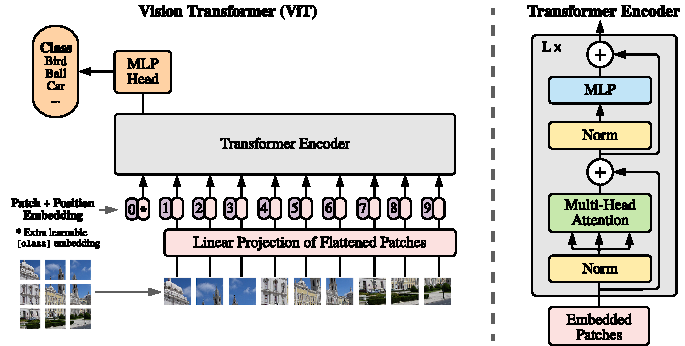
\includegraphics[width=0.8\columnwidth,keepaspectratio]{images/vision_transformer.pdf}
      \caption{\small Transformador visual. Fonte: \textcite{dosovitskiy2020image}.}
      \label{fig:vision_transformer}
\end{figure}

No contexto de codificadores visuais, a classificação não é necessária, já que a saída do codificador se constitui nas incorporações processadas. Sendo assim, a
incorporação extra de classificação e o \ac{MLP} final podem ser desconsiderados \cite{dubey2024llama}.

\subsection{Projetor de Entrada}

Esse componente faz o alinhamento entre o espaço de incorporações geradas pelo codificador e o espaço de incorporações do \ac{LLM}, podendo utilizar um \ac{MLP} ou um
mecanismo de \textit{cross-attention}. A principal diferença de \textit{cross-attention} para \textit{self-attention} nesse contexto está no uso dos vetores de
\textit{key} provenientes do codificador para o cálculo da atenção no transformador do \ac{LLM} \cite{mllm_survey_2024}.

\subsection{Treinamento}

Com base no trabalho de \textcite{mllm_survey_2024}, pode-se dividir o treinamento de \acp{MLLM} em pré-treinamento e \textit{instruction-tuning}. Porém, esse processo
normalmente envolve a utilização de um \ac{LLM} pré-treinado e alinhado, portanto, o treinamento de um \ac{LLM} será considerado como a primeira etapa.

\subsubsection{Treinamento de LLMs}

\acp{LLM} requerem grandes volumes de dados para serem treinados, sendo que esses dados textuais precisam ser tratados antes de serem usados. O tratamento envolve a
remoção de informações falsas, textos duplicados, ruídos e de dados sem valor para o treinamento. Além disso, os vieses e desbalanceamentos também são reduzidos nesse
processo \cite{llm_survey_2024}.

\subsubsubsection{Pré-treinamento de LLMs}

O pré-treinamento é a primeira etapa de treinamento de um \ac{LLM}. Normalmente o modelo é treinado sobre um grande volume de texto não classificado de forma
auto-supervisionada. A modelagem auto-regressiva e a modelagem mascarada são duas formas comuns de realizar o pré-treinamento.

Na modelagem auto-regressiva, o modelo tenta prever o próximo \textit{token} a partir de uma sequência de \textit{tokens}. O \textit{token} previsto é comparado com o
\textit{token} esperado, assim, o modelo tentará minimizar os erros. Essa modelagem é mais adequada para \acp{LLM} que usam apenas decodificadores, devido ao fato da
predição ser baseada apenas nos \textit{tokens} antecessores ao \textit{token} previsto.

A modelagem mascarada se consiste no treinamento baseado na previsão de partes ocultas de um texto. Diferentemente da modelagem auto-regressiva, este método utiliza
todos os \textit{tokens} do texto para realizar a previsão.

\subsubsubsection{Alinhamento} \label{sec:alinhamento}

Com o pré-treinamento, os \acp{LLM} conseguem gerar e classificar textos, mas ainda é necessário alinhar o comportamento do modelo com as expectativas de seus usuários.
Com o método \ac{RLHF}, os textos gerados são avaliados por humanos, recebendo uma pontuação. Assim, é possível ajustar o modelo para que as respostas tenham
pontuações melhores. Outro método comum é o \ac{RLAIF}, que integra um modelo já alinhado ao que está em treinamento, realizando os ajustes necessários.

\subsubsection{Pré-treinamento}

O pré-treinamento de um \ac{MLLM} normalmente evolve o travamento dos codificadores de modalidade e do \ac{LLM}, fazendo com que somente o projetor seja treinado. Em
alguns casos, o codificador de modalidade também é destravado, permitindo um treinamento mais completo. O objetivo nessa etapa é alinhar o codificador de modalidade com o
\ac{LLM}. No contexto de modelos visuais, o pré-treinamento faz o uso de um grande volume de pares de imagens e textos, sendo que os textos descrevem o conteúdo das
imagens \cite{mllm_survey_2023}.

\subsubsection{Instruction-tuning}

Essa etapa se consiste na melhoria do modelo para atender melhor às expectativas dos usuários e obter uma capacidade melhor na resolução de problemas envolvendo tarefas
multimodais, sendo uma etapa similar à de alinhamento discutida na \autoref{sec:alinhamento}.

No contexto de modelos visuais, \textit{Instruction-tuning} pode ser feita inicialmente com \ac{SFT}, usando imagens e textos em um formato de pergunta e resposta, em
que uma pergunta é feita sobre a imagem. Depois da aplicação de \ac{SFT}, é possível usar \ac{RLHF} para continuar o aprimoramento do modelo \cite{mllm_survey_2024}.

\subsubsection{Fine-Tuning}

O \textit{fine-tuning} é uma etapa de treinamento que pode ser realizada para melhorar o desempenho do modelo com relação a dados específicos ou sobre um domínio de
conhecimento. Técnicas de \textit{fine-tuning} eficientes, como as baseadas em \ac{PEFT}, oferecem uma forma de adaptação de modelos com um custo computacional
elativamente menor. Dentre várias técnicas, uma das mais populares é o \ac{LoRA} \cite{llm_survey_2023}.

\subsubsubsection{LoRA}

Essa técnica, proposta por \textcite{hu2021lora}, consiste-se em explorar o \textit{rank} intrínseco, um conceito baseado em dimensionalidade intrínseca, introduzindo
matrizes treináveis menores de baixo \textit{rank} ao \ac{MLLM}, deixando as matrizes originais intactas durante o treinamento. Assim que treinadas, essas matrizes são
adicionadas às originais.

O \textit{rank} de uma matriz é o número de colunas ou linhas linearmente independentes que a matriz possui. Ele também corresponde à dimensão do espaço vetorial
gerado pelas colunas ou linhas. O \textit{rank} intrínseco se trata do menor \textit{rank} que a matriz pode ter no treinamento sem haver uma grande perda de desempenho.

Assim, pode-se resumir que com base em uma matriz \begin{math}W_0\end{math} do modelo, tal que \begin{math}W_0 \in \mathbb{R}^{d \times k}\end{math}, é possível
representá-la em uma forma decomposta \begin{math}W_0 + \Delta W\end{math} em que \begin{math}\Delta W = BA\end{math}, tal que
\begin{math}B \in \mathbb{R}^{d \times r}\end{math} e \begin{math}A \in \mathbb{R}^{r \times k}\end{math}, sendo que \begin{math}r \ll min(d, k)\end{math}. A matriz
\begin{math}W_0\end{math} é travada enquanto as matrizes \begin{math}A\end{math} e \begin{math}B\end{math} são treináveis. A matriz \begin{math}A\end{math} é
inicializada com uma distribuição gaussiana aleatória e a \begin{math}B\end{math} é inicializada como zero. Na \autoref{fig:lora} é apresentada uma representação visual
do \ac{LoRA} com a expressão \begin{math}h = W_0x + BAx\end{math}.

\begin{figure}[ht]
      \centering
      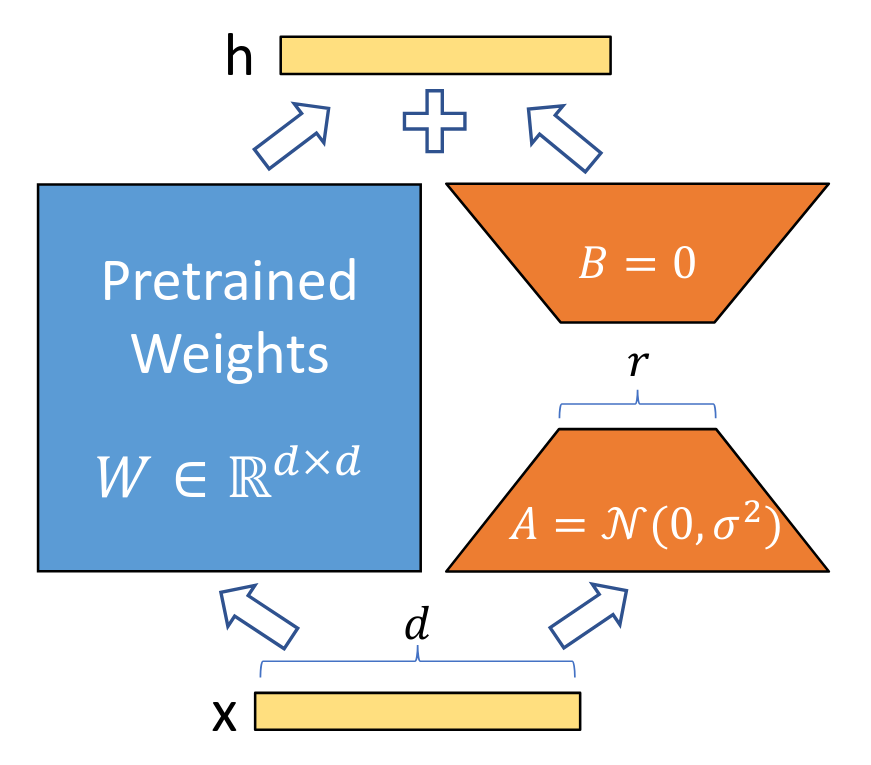
\includegraphics[width=0.35\columnwidth,keepaspectratio]{images/lora.png}
      \caption{\small Representação do \ac{LoRA} com as matrizes \begin{math}W_0\end{math}, \begin{math}A\end{math} e \begin{math}B\end{math}. Fonte:
            \textcite{hu2021lora}.}
      \label{fig:lora}
\end{figure}

\subsubsubsection{QLoRA} % TODO: Explicar mais no futuro, talvez?

É possível usar também a quantização para acelerar o \textit{fine-tuning}. A quantização se trata da redução da precisão numérica durante o treinamento. Uma técnica que
utiliza este conceito é o \ac{QLoRA}, proposta por \textcite{qlora}. Nessa técnica, é usado o tipo \ac{NF4} no armazenamento das matrizes pré-treinadas, sendo que os
valores em \ac{NF4} são convertidos para \textit{BFloat16} durante os cálculos. Além disso, também são usados otimizadores paginados e dupla quantização.

\section{LLaMA 3}

A família de modelos \ac{LLaMA}-3 é composta por \acp{LLM} e \acp{MLLM} desenvolvidos pelos pesquisadores da \textit{Meta AI}. Em particular, este trabalho focará no
modelo multimodal \ac{LLaMA}-3.2, que possui as variantes com 11 e 90 bilhões de parâmetros disponíveis \cite{dubey2024llama}.

O \ac{LLM} base do \ac{LLaMA}-3.2 utiliza um transformador decodificador que possui algumas diferenças em relação à arquitetura original de \textcite{transformer}, as
maiores diferenças já existem desde os modelos \ac{LLaMA} e \ac{LLaMA}-2 e podem ser elencadas com base no trabalho de \textcite{touvron2023llama}:

\begin{itemize}
      \item \textbf{Pré-normalização}: As subcamadas são pré-normalizadas, em vez de serem normalizadas posteriormente;
      \item \textbf{Normalização}: A função de normalização usada é a \ac{RMSNorm};
      \item \textbf{Função de ativação}: Na subcamada de \textit{feed-forward}, a função de ativação é a \ac{SwiGLU}, em vez de \ac{ReLU};
      \item \textbf{Codificação posicional}: A codificação posicional é feita com \ac{RoPE}, em vez da codificação absoluta;
      \item \textbf{\acs{GQA}}: \ac{GQA} é utilizado é com 8 cabeças de chave-valor para melhorar a velocidade de inferência e reduzir o tamanho dos \textit{caches} de
            chave-valor durante a decodificação;
      \item \textbf{Máscara de atenção}: Uma máscara é utilizada para impedir o relacionamento entre diferentes documentos de uma mesma entrada;
      \item \textbf{Vocabulário}: O vocabulário de \textit{tokens} usado possui 128 mil \textit{tokens}.
\end{itemize}

A \autoref{tab:llama3_architecture} apresenta alguns parâmetros das variantes do \ac{LLM}.

\begin{table}[ht]
      \caption{\small Características das variantes do \ac{LLaMA}-3}
      \centering
      \begin{tabular}{l|ccc}
            \hline
                                                   & 8B                                                                   & 70B                                      & 450B                                   \\ \hline
            Camadas do transformador               & 32                                                                   & 80                                       & 126                                    \\
            Dimensão das incorporações             & 4096                                                                 & 8192                                     & 16384                                  \\
            Dimensão da rede \textit{feed-forward} & 14336                                                                & 28672                                    & 53248                                  \\
            \textit{fAttention heads}              & 32                                                                   & 64                                       & 128                                    \\
            \textit{fKey / Value heads}            & 8                                                                    & 8                                        & 8                                      \\
            Taxa máxima de aprendizado             & \begin{math}3 \times 10^{-4}\end{math}                               & \begin{math}1.5 \times 10^{-4}\end{math} & \begin{math}8 \times 10^{-5}\end{math} \\
            Função de ativação                     & \multicolumn{3}{c}{\ac{SwiGLU}}                                                                                                                          \\
            Tamanho do vocabulário                 & \multicolumn{3}{c}{128000}                                                                                                                               \\
            Codificação posicional                 & \multicolumn{3}{c}{\ac{RoPE}\begin{math}(\theta = 500000)\end{math}}                                                                                     \\ \hline
      \end{tabular}
      \label{tab:llama3_architecture}
      \fonte{\textcite{dubey2024llama}}
\end{table}

O codificador visual utilizado é baseado no transformador visual de \textcite{dosovitskiy2020image}, sendo usada a variante \ac{ViT}-H/14 com modificações extras, como
a adição de extração de características multicamadas e de 8 camadas de \textit{gated self-attention}, deixando o codificador com um total de 850 milhões de parâmetros.

O projetor de entrada, referenciado como adaptador de visão no trabalho de \textcite{dubey2024llama}, se baseia em \textit{cross-attention} entre as camadas de
codificação do codificador visual e as camadas de decodificação do \ac{LLM}. Mais especificamente, é aplicada uma camada de \textit{cross-attention} a cada quarta camada
do \ac{LLM}. Essas camadas também utilizam \ac{GQA} para melhorar o desempenho.

Além de imagens, o \ac{LLaMA}-3.2 também pode operar com vídeos e áudios. A \autoref{fig:llama} apresenta a arquitetura multimodal do modelo.

\begin{figure}[ht]
      \centering
      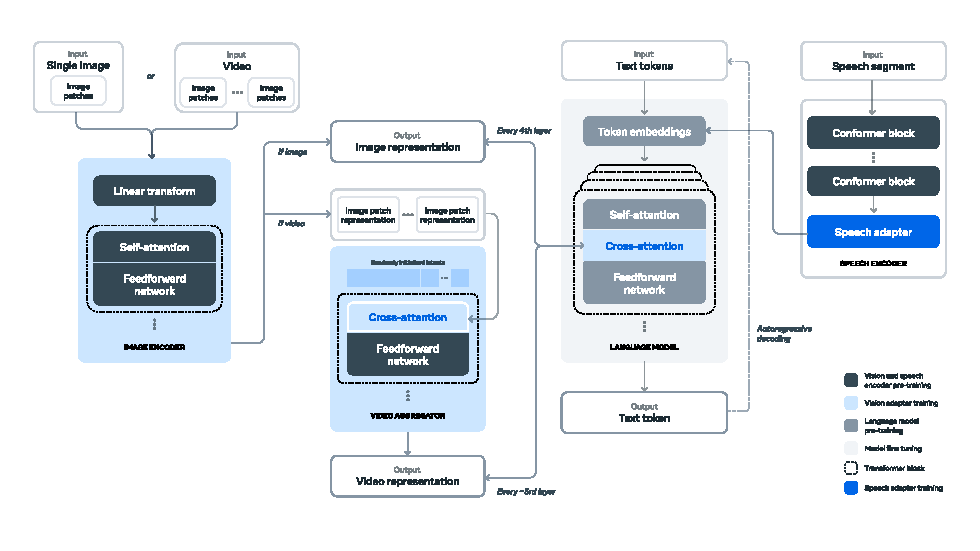
\includegraphics[width=1.0\columnwidth,keepaspectratio]{images/llama.pdf}
      \caption{\small Arquitetura multimodal de imagem e vídeo do \ac{LLaMA}-3.2. Fonte: \textcite{dubey2024llama}.}
      \label{fig:llama}
\end{figure}
